\subsection{API Test Runs}
These are the tests for the restful API. The API acts as a means of communicating with the database. In order to do so, certain requests - either GET, POST, PUT or DELETE - are sent to an address; in this case, \textit{/api/quizzes}. The API then looks at the request type that was sent, along with any other data that came with it, and performs the appropriate operation, be that showing a list of all quizzes, showing a specific quiz, or updating a quiz.

\subsubsection{api.spec.js} % (fold)
\label{ssub:api_spec_js}
\lstinputlisting[language=javascript, caption=Unit tests for the API.]{../test/api.spec.js}
\begin{figure}[h!]
  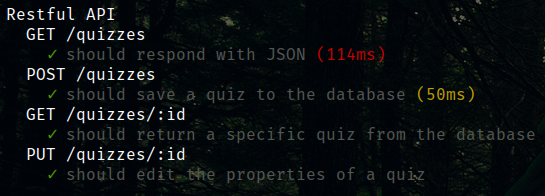
\includegraphics[scale=0.55]{testing/api/api}
  \caption{Test outcome for api.spec.js 1}
\end{figure}
% subsubsection api_spec_js (end)

As can be seen by the little green ticks, all the different HTTP methods passed, proving that the API is working correctly, and thereby allowing requests to be sent from throughout the application. \textit{Success.}

